

The conservation equations of mass and momentum, derived using \ref{eq:avg_dt_dq_alpha_tot} and \ref{eq:hybrid_avg_dt_chif} yield the same as the classical hybrid models derived in previous studies such as \citet{jackson1997locally} and \citet{zhang1997momentum} among others.
Therefore, it will not be discussed further as it does not contribute any relevant information to the current study.
Instead, in the subsequent analysis, we consider as known quantities : the fluid phase fraction $\phi_1$;
the particle number density $n_p$; the continuous phase-averaged velocity $\oneavg{\textbf{u}}$; and particle-average velocity $\pnnavg{\textbf{u}_\alpha}$. 
Which implies that the equations of conservation of mass and momentum for both the continuous and dispersed phase have been solved a priori, providing the values of these variables as known quantities.
Additionally, it also implies that the closure terms in the momentum equation, such as the mean interphase drag force $\pnnavg{\textbf{f}_\alpha}$ and others terms must be closed. 
However, those terms might depend on the higher moments of the particle phase, in which case it is crucial to provide a first-order moment equation. 
Therefore, the primary objective of this section is to emphasize the significance of the first-moment equations derived from \ref{eq:avg_dt_dQ_alpha_tot}, as they are often overlooked and underutilized in the literature.
In this section we stay succinct while providing the minimum level of understanding of the problem at hand.
Hence, we will not entirely deal with the closure problem of these first-order moments equations, but rather we focus on their derivation and interpretation. 

\subsection{Solid axis symmetric particle suspension}

% Let's start by the second moment of mass averaged equation.
Let's examine the scenario of a mono-disperse axissymmetric suspension of solid particles, such as ellipsoid or cylinders.
Let the vector $\textbf{p}$ denote the unit vector representing the orientation of the particle along its main axis of inertia. 
Then, the second moment of mass can be written as $\mathcal{M}_\alpha =  \textbf{pp} (M_\alpha^{||} - M_\alpha^\bot) +  \textbf{I} M_\alpha^\bot$, where $M_{\bot}$ and $M_{||}$ represent the coefficients corresponding to the principal directions of the particles' mass distribution.
It is well-established that $\pnnavg{\textbf{f}_\alpha}$ exhibits a significant dependence on the orientation of the particle \citep{kim2013microhydrodynamics}.
Therefore, despite being a second-order moment, the particle field $\mathcal{M}_\alpha$ is indispensable to solve the mono-disperse axissymmetric suspension problem.

Averaging the second-order moment of mass yields, $\pnavg{\mathcal{M}_\alpha} =  \textbf{A} (M_\alpha^{||} - M_\alpha^\bot) +  \textbf{I} M_\alpha^\bot$ where $\textbf{A}$ is the orientation tensor defined as $\textbf{A} = \avg{\delta_\alpha\textbf{pp}} = \pnavg{\textbf{pp}}$.
Then, let's express the internal motion of a solid particle by : $\textbf{u}_2(\textbf{x}_\alpha) = \textbf{u}_\alpha + \textbf{r}\times \omega_\alpha$ where $\omega_\alpha$ represents the angular velocity of the particle.
It follows the expression of the stretching of momentum : $\mathcal{S}_\alpha = (M_\alpha^{||} - M_\alpha^\bot) \left(
    \omega_\alpha \times
    \textbf{pp}
    + \textbf{pp} \times \omega_\alpha
\right)$. 
Subsequently,  we can easily derive the transport equation for $\textbf{A}$ by averaging \ref{eq:dt_M_alpha} and using the previous expressions for $\mathcal{M}_\alpha$ and $\mathcal{S}_\alpha$.
The resulting equation is given by~:
\begin{equation}
    \pddt (n_p\textbf{A})
    + \div (
        \pnnavg{\textbf{u}_\alpha}\textbf{A}
        + \mathbf{\Sigma}
        )
    =
    \pnavg{\textbf{pp} \times \omega_\alpha}
    + \pnavg{\omega_\alpha \times \textbf{pp}},
    % + \pnavg{\textbf{pp}' \times \omega_\alpha'}
    % +\pnavg{\omega_\alpha' \times \textbf{pp}'}
    \label{eq:avg_dt_M_alpha}
\end{equation}
where $\mathbf{\Sigma} = \pnavg{\textbf{u}'_\alpha(\textbf{pp})'}$ is the covariance term between the fluctuation of the velocity and the orientation tensor.
We recall that the definition of the fluctuation notation is provided by the expression from \ref{eq:def_fluctu}.
At this stage we need to find closure for both terms on the RHS of \ref{eq:avg_dt_M_alpha}. 
Therefore, we assume torque free rigid particle in to Stokes flow, where we can utilize Jeffery's equation \citep{guazzelli2011}.
It reads,
\begin{equation}
    \omega_\alpha \times \textbf{p}
    = \mathbf{\Omega}\cdot\textbf{p}
    + \beta\left(
        \textbf{E}\cdot \textbf{p}
        - \textbf{E} : \textbf{ppp}
    \right),
    \label{eq:jefferey}
\end{equation}
with $\textbf{E}$ and $\mathbf{\Omega}$ being the symmetric and antisymmetric parts of the bulk velocity gradient, respectively, such that $\grad\avg{\textbf{u}}=\textbf{E}+\mathbf{\Omega}$.
The coefficient $\beta$  is a constant related to the aspect ratio of the particle.
Finally, by substituting the RHS terms of \ref{eq:avg_dt_M_alpha}, by using \ref{eq:jefferey}, we arrive at the closed form of the second moment of mass equation~:
\begin{equation}
    \pddt \textbf{A}
    + \div (
        \pnnavg{\textbf{u}_\alpha}\textbf{A}
    )
    =
    \mathbf{\Omega} \cdot \textbf{A}
    - \textbf{A} \cdot \mathbf{\Omega}
    + \beta\left[
        \textbf{E} \cdot \textbf{A}
        -\textbf{A} \cdot \textbf{E}
        - \textbf{E} : \mathbb{A}
    \right]
    - \div \mathbf{\Sigma}
    \label{eq:hybrid_avg_dt_pp}
\end{equation}
where the fourth-order tensor $\mathbb{A}$, is defined as $\mathbb{A} = \pnavg{\textbf{pppp}}$.
In \citet{wang2008objective} they derive \ref{eq:hybrid_avg_dt_pp} by the means of kinetic theory, based on \ref{eq:jefferey} and the fact that $\ddt \textbf{p} = \omega_\alpha \times \textbf{p}$ (Equation (3) of their article).
Their equation is similar to \ref{eq:hybrid_avg_dt_pp} except that their employ a phenomenological closure for the term, $\div \mathbf{\Sigma}$, which account for particles interactions.
Anyhow, we showed how it is possible to derive the orientation tensor conservation equation, commonly used in fiber field theory, from the second-order moments of mass's equation. 

\subsection{Contaminated bubbly flows}

Let's consider a mono-disperse rising bubbly flow without phase transfer made of spherical particles of radius $a$, that is contaminated by soluble surfactants.
We denote $c_1$ as the molar concentration of surfactant in the continuous phase, and $c_I$ as the surface molar concentration of surfactant on the bubbles' interface.
Additionally, we make the assumption that there is no transport of surfactant inside the dispersed phase. 
This assumption is reasonable in the case of air bubbles.
According to the Langmuir model \citep{pesci2018computational}, we have the relationship:
\begin{equation}
    \sigma
    = \sigma_0
    + RT c_I^\infty
    \ln\left(1-\frac{c_I}{c_I^\infty}\right)
    \label{eq:sigma_def}
\end{equation}
where $R$ is the universal gas constant, $T$ the absolute temperature, $c_I^\infty$ the saturated surfactant concentration, and $\sigma_0$ to the surface tension coefficient when the surfaces are completely clean.
On the other hand, as represented on \ref{fig:contaminated_bubbles}, during the rise of a bubble in the flow, the surfactants are transported along the droplets surface, which in turns create a stagnant cap in the opposite direction of the droplet velocity.
According to \ref{eq:sigma_def} the possibly inhomogeneous concentration field, $c_I$, generates a spatially non-constant surface tension coefficient $\sigma$.
Additionally, remark that the gradient of the surface tension generates additional Marangoni forces as represented in \ref{fig:contaminated_bubbles} and expressed by \ref{eq:surface_tension}.
These additional surface tension forces alter the flow behavior in the vicinity of the droplet's surface.
Therefore, this alteration in surface tension impacts the local hydrodynamic, but also induce a change in the shape of the particle through both, \ref{eq:dt_S_alpha} and \ref{eq:dt_M_alpha}.
As a result, the drag force and drift velocity experienced by a rising bubble or droplet are directly influenced by the surfactant concentration and its distribution over the surface \citep{pesci2018computational}.
Moreover, a recent study by \citet{kentheswaran2022direct} have demonstrated that the mean concentration and distribution of surfactants on the bubbles' surface also have a significant impact on the mass transfer rate between the dispersed and continuous phases.
Therefore, in this example we present an averaged hybrid model that aims to predict the evolution of the averaged surfactant concentration in the bulk $\oneavg{c}$, and the averaged surfactant on the surface of the particle, defined by, $C_{\alpha}= \frac{1}{s_\alpha}\int c_I d\Sigma$.
Additionally, we also provide the moment equation for the center of the distribution of $c_I$, which is defined as $\textbf{r}_\alpha = \frac{1}{s_\alpha C_\alpha}\int_{\Sigma_\alpha} \textbf{r}c_Id\Sigma$.
Note that $\int_{\Sigma_\alpha} \textbf{r}c_Id\Sigma =  \frac{s_\alpha}{4 \pi}\int_{\Sigma_\alpha} \gradI (c_I) d\Sigma$, thus $\textbf{r}_\alpha$ can also be interpreted as the mean gradient of surfactant on a particle's surface.
Consequently, by the mean of \ref{eq:sigma_def}, $\textbf{r}_\alpha$ is also related to the resultant of Marangonie forces on a particle's surface.  
A graphical representation of $\textbf{r}_\alpha$ is given \ref{fig:contaminated_bubbles}.

\begin{figure}[h!]
    \centering
    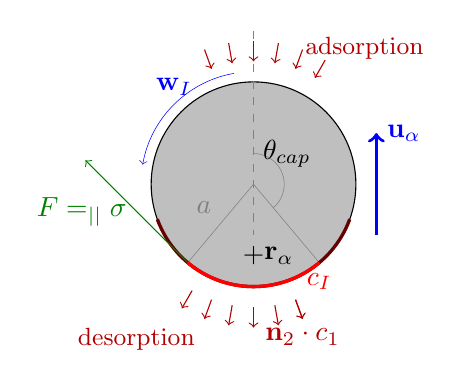
\begin{tikzpicture}[scale =1.3]
        \draw[fill=lightgray](0,0) circle (1);
        \draw[very thin,gray](230:1)--(0,0)node[midway,above left]{$a$}--(310:1);
        \draw[very thin,gray](0,0)++(310:0.3) arc (-50:90:0.3)node[right,black]{$\theta_\text{cap}$};
        \draw[very thin,blue,->](0,0)++(100:1.1) arc (100:170:1.1)node[midway,above]{$\textbf{w}_I$};
        \draw[very thick,red!40!black](0,0)++(200:1) arc (200:340:1);
        \draw[very thick,red](0,0)++(230:1) arc (230:310:1)node[below]{$c_I$};
        \draw[very thick,dashed](0,0)++(0,-0.7)node{$+$}node[right]{$\textbf{r}_\alpha$};
        \draw[very thick,blue,->](1.2,-0.5)--++(0,1)node[right]{$\textbf{u}_\alpha$};
        \draw[dashed,gray](0,1.5)--++(0,-2);
        \draw[red,->,green!50!black](230:1)--++(-1,1)node[midway,left]{$F = \grad_{||} \sigma$};
        \foreach \t in {110,100,90,80,60}{
            \draw[red!70!black, ->](\t:1.4)--++(\t:-0.2);
            \draw[red!70!black, ->](\t:-1.2)--++(\t:-0.2);
        }
        \draw[red!70!black, ->](70:1.4)--++(70:-0.2)node[above right]{\small adsorption};
        \draw[red!70!black, ->](70:-1.2)--++(70:-0.2)node[below left]{\small desorption};
        \draw[red!70!black, ->](110:-1.2)--++(110:-0.2)node[below]{$\textbf{n}_2 \cdot \grad c_1$};
    \end{tikzpicture}
    \hspace{2em}
    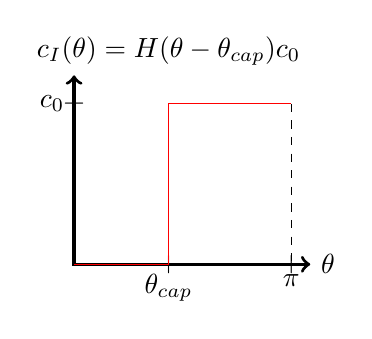
\begin{tikzpicture}[scale =1.2]
        \draw[very thick,<->](0,2)--(0,0)--(2.5,0)node[right]{$\theta$};
        \draw(1,0)node{$+$}node[below]{$\theta_{cap}$};
        \draw(1,2)node[above]{$c_I(\theta) = H(\theta- \theta_{cap}) c_0$};
        \draw[very thin,dashed](2.3,1.7)--(2.3,0);
        \draw[thin,red](0,0)--++(1,0)--++(0,1.7)--++(1.3,0);
        \draw(2.3,0)node{$+$}node[below]{$\pi$};
        \draw(0,1.7)node{$+$}node[left]{$c_0$};
    \end{tikzpicture}
    \caption{ (left) Scheme of the stagnant-cap regime of a rising contaminated bubble in a quiescent liquid. 
    (right) Hypothetical profile of the surface concentration $c_I$ in terms of the azimuthal coordinate $\theta$. }
    \label{fig:contaminated_bubbles}
\end{figure}


To derive the microscopic scale conservation equation of $c_I$ and $c_1$ we set $f_1 = c_1$ and $f_I = c_I$ in \ref{eq:dt_f_k} and \ref{eq:dt_f_I}, respectively.
Additionally, we assume that the  diffusive flux follow a Fick's law model, i.e.  $\mathbf{\Phi}_1 = D\grad c_1$ and $\mathbf{\Phi}_I = D_I\gradI c_I$,
where the constant,  $D$ and $D_I$ are the volumetric and surface diffusion coefficient, respectively.
Note that this diffusive model remains true under the assumption of dilute species concentration in both the liquid and at the interface.
\tb{The diffusive terms change in function of the regime : dilute concentration / saturated concentration, in which case $D\grad c_1 = f(c_I)$, it is worth going into that mush details ? no.}
Moreoverer, We do not consider chemical reaction or any other source term, i.e. $\textbf{S}_k = 0$ and $\textbf{S}_I=0$. 
Then, by injecting these terms in \ref{eq:dt_f_k} and \ref{eq:dt_f_I} we obtain these conservation equations : 
\begin{align}
    \pddt c_1
    + \div (\textbf{u}_1 c_1)
    &= \div (D \grad c_1)
    \;\;\; \text{in} \;\;\; \Omega_1,\\
    \pddt c_I
    + \divI (\textbf{u}_I c_I)
    &= \divI (D_I \gradI c_I)
    - (D \grad c_1)\cdot \textbf{n}_2
    \;\;\; \text{on} \;\;\; \Sigma,
    \label{eq:dt_c_I}
\end{align}
In agreement with \citet{pesci2018computational,manikantan2020surfactant}.
We recognize that the last term of \ref{eq:dt_c_I}, namely $D(\grad c_1 ) \cdot \textbf{n}_2$, turns out to be the \textit{Kinetically controlled sorption} boundary condition \citet{pesci2018computational,manikantan2020surfactant} which arise naturally in our model.
Specifically, it represents the adsorption and desorption flux between the bulk and the surface, as represented in \ref{fig:contaminated_bubbles}.
% For clarity remark that for exemple Equation (3.9) of \citet{manikantan2020surfactant} corresponds to the \textit{two-fluid} formulation of \ref{eq:dt_c_I} with a Fick's law model. 
Note that this exchange term is reduced to a contribution from the continuous phase since we assume no surfactant into the dispersed phase. 
Now that we clearly derived the microscale equation in both phases, we can easily derive the averaged equations of conservation using the hybrid model presented \ref{sec:averaged_eq}.

For a better understanding of the following equations, we now describe the steady-state kinetics that can be reached for an isolated bubble in a contaminated flow, as illustrated on \ref{fig:contaminated_bubbles}.
This will serve as a reference for the subsequent discussion.
We first assume that the transport of surfactants on the surface, represented  by the term  $\textbf{w}_I c_I$, is much greater than the other diffusive processes, such as $D\grad c_1$ and $D_I\gradI c_I$ as well as the adsorption-desorption effects. 
In this regime, the concentration of surfactant that enters from the forward-surface, due to adsorption, is advected almost instantaneously to the downward region of the particle where some of it evaporates due to desorption. 
This form an accumulation of surfactant on the downward region of the particle's surface.
At a certain point of equilibrium, the adsorption and desorption flux balance each other, leading to the steady-state kinetic of $c_I$, and the stagnant cap is stabilized to a concentration $c_0$. 
In this situation, we can consider that $c_I$ follows a constant sharp distribution along the azimuthal coordinate of the particle's surface.
Specifically, we model $c_I(\theta) = H(\theta - \theta_{cap}) c_0$ where $H$ is the Heaviside function and $\theta_{cap}$ is the angle at which the stagnant cap is formed, see \ref{fig:contaminated_bubbles}.
This assumption might seem unrealistic, nevertheless in the steady-state regime, it is approximately consistent with the observations \citep{kentheswaran2022direct}.
% In these condition the physical meaning of the first moment, $\textbf{r}_\alpha$, becomes clearer. 
From the expression of $c_I$ we deduce : $C_\alpha = \frac{c_0}{2}(1+\cos\theta_{cap})$ and $\textbf{r}_\alpha = \frac{a}{2} (\cos\theta_{cap} -1)\textbf{e}$ where $\textbf{e}$ is the unit vector in the direction of the relative velocity between the particle and the continuous phase velocity.
Thus, the knowing $\textbf{r}_\alpha$ can leads use to $\theta_{cap}$. 
This is crucial information, since the drag forces term and mass transfer closure terms are usually derived in terms of $\theta_{cap}$, such as in the following studies : \citet{sadhal1983stokes} and \citet{kentheswaran2022direct}. 

Now that the problem has been properly formulated, we can begin the derivation of the averaged equations.
The phase-averaged conservation equation for the mean concentration of surfactant in the bulk $\oneavg{c}$, is derived using \ref{eq:avg_dt_chi_f}.
It reads as,
\begin{equation}
    \pddt (\phi_1 \oneavg{c})
    + \div (\phi_1 \oneavg{c} \oneavg{\textbf{u}_1})
    = D \grad^2 (\phi_1\oneavg{c})
    - \pnavg{j_\alpha}
    +  \div \mathbf{\Sigma}_c,
    \label{eq:hybrid_avg_dt_c_1}
\end{equation}
where $j_\alpha$ is the exchange term with the dispersed phase given by,
\begin{equation*}
    j_\alpha
    =\int_{\Sigma_\alpha}
    (D\grad c_1 )
\cdot \textbf{n}_2d\Sigma,
\end{equation*}
which corresponds to the resultant of the surfactant exchange including adsorption and desorption flux.  
In the steady-state regime, when the adsorption flux balance the desorption flux,  the surfactant on the surface of the bubble can be considered as globally insoluble since $j_\alpha=0$ even through $D(\grad c_1 ) \cdot \textbf{n}_2$ may not be locally zero. 
This \textit{globally insoluble} assumption has been used in numerous studies to neglect the adsorption-desorption fluxes. 
The vector $\mathbf{\Sigma}_c$ in \ref{eq:hybrid_avg_dt_c_1}, has the following expression,
\begin{equation}
    \mathbf{\Sigma}_c
    =
     \pnavg{\textbf{J}_\alpha}
    - \pnavg{\frac{D}{a}\int_{\Sigma_\alpha}  c_1 \textbf{r} d\Sigma}
    - \phi_1\oneavg{c'_1\textbf{u}_1'},
    \label{eq:B_def}
\end{equation}
where the higher order terms have been neglected. 
The first term on the RHS of \ref{eq:B_def} corresponds to the first moment of the surfactant flux, namely $\textbf{J}_\alpha = \int_{\Sigma_\alpha} \textbf{r}
(D\grad c_1)\cdot \textbf{n}_2d\Sigma$.
It can be interpreted as the vector representing the mean direction and magnitude of the surfactant flux going in and out the surface of the droplets.
In the stagnant cap regime, this term is therefore non-zero since a mean flux is still present even through its resultant is null, i.e. $j_\alpha=0$.
In the reference frame of the particles, $\textbf{J}_\alpha$ account for the mean flux of species concentration induced by the presence of the particles, due to adsorption and desorption phenomena. 
The second term of \ref{eq:B_def} comes from the inclusion of $\phi_1$ inside the Laplacian operator in \ref{eq:hybrid_avg_dt_c_1}.
It is the first moment of $c_1$ over the droplets surface, thus it is the mean position of the continuous phase surfactant concentration over the droplet surface.
For a constant distribution $c_1$ at the bubbles interface, this vector would be zero. 
Finally, The last term of \ref{eq:B_def}, $\phi_1\oneavg{c'_1\textbf{u}_1'}$, represents the diffusive term due to the correlation of $c'_1$ with $\textbf{u}_1'$.
Overall, $\mathbf{\Sigma}_c$ is a balance between the first moment of the fluxes and the first moment of the bulk concentration, minus a contribution from the fluctuations.
Note that $\mathbf{\Sigma}_c$ appear under the divergence operator in \ref{eq:hybrid_avg_dt_c_1}, thus it will be relevant only in highly inhomogeneous cases. 
% At this stage of the research it is hard to predict the form of these closure terms. 
% Nevertheless, we know that the closure for $j_\alpha$ and $\mathbf{\Sigma}_c$ are function of the mean surface concentration $C_\alpha$ and its center of distribution $\textbf{r}_\alpha$.
% Indeed, the exchange term $\grad c_1$ which is function of the local concentration $c_I$ at surfactant saturation \citep{manikantan2020surfactant}. 
% Thus, an equation for $C_\alpha$ and a moment equation for $\textbf{r}_\alpha$ are needed. 

Regarding the equations dispersed phase, we start by the transport equation of the mean surface surfactant concentration $C_\alpha$.
From \ref{eq:avg_dt_dq_alpha_tot} the averaged conservation equation of $C_\alpha$ is straightforward to obtain and reads as,
\begin{equation}
    \pddt (\pnavg{C_\alpha})
    + \div (\pnavg{\textbf{u}_\alpha} \pnnavg{C_\alpha})
    =
    \frac{\pnavg{j_\alpha}}{s_\alpha}
    - \div (\pnavg{\textbf{u}_\alpha' C'_\alpha}).
    \label{eq:avg_dt_dC_alpha}
\end{equation}
As shown by this equation, the evolution of the mean concentration of surfactant on the particles' surface is driven by the exchange term $j_\alpha$ and the fluctuation term $\pnnavg{\textbf{u}_\alpha' C_\alpha'}$. 
The latter term is the covariance between the velocity of the particles and their mean surfactant concentration. 
It is known that the rising velocity of a bubble is greatly correlated with its mean surfactant concentration \citet{kentheswaran2022direct} thus it might be of a certain importance. 
Again, this term is under the divergence operator it will be therefore important only in non-homogeneous cases. 
Anyhow, this term must be further investigated.

We now derive an equation for the mean position of the surfactant, $\pnnavg{\textbf{r}_\alpha}$.
This is done by deriving the equation of the first moment, $s_\alpha C_\alpha \textbf{r}_\alpha$ using \ref{eq:dt_Q_alpha_tot}. 
Then, we reformulate the equation using  the relation, $\ddt (s_\alpha C_\alpha \textbf{r}_\alpha) = s_\alpha C_\alpha\ddt \textbf{r}_\alpha+ s_\alpha \textbf{r}_\alpha\ddt C_\alpha $ and  $\ddt C_\alpha = j_\alpha$. 
Finally,  we apply the average process which leads us to~:
\begin{multline}
    \pddt (\pnavg{\textbf{r}_\alpha})
    + \div (\pnavg{\textbf{u}_\alpha}\pnnavg{\textbf{r}_\alpha})
    =
    - \div (\pnavg{\textbf{u}'_\alpha\textbf{r}'_c})\\
    + \frac{n_p}{s_\alpha}\pnnavg{
        \frac{1}{C_\alpha}\left[
            \int_{\Sigma_\alpha} 
            \left[
                c_I \textbf{w}_I
                - D_I (\gradI c_I)
            \right] d\Sigma
            +\textbf{J}_\alpha
            - \textbf{r}_\alpha j_\alpha
        \right]
    }.
    \label{eq:avg_dt_dr_alpha_tot}
\end{multline}
The diffusive term $\pnavg{\textbf{u}'_\alpha\textbf{r}'_c}$ which represents the flux generated by the correlation between the mean surfactant distribution on the particles' surface and the velocity of the particles. 
Again, this term might be relevant since, as mentioned previously, the rising velocity is highly dependent on $\theta_{cap}$.
Then, the first term on the second line is the contribution of the averaged surface advection of $c_I$ along the particles' surface. 
The second term accounts for the diffusion of surfactants over the droplet surface, which acts against the formation of a sharp distribution of surfactants.
However, the contribution of this term is likely negligible based on the values of the diffusive surface coefficient, as discussed in \citet{valkovska2000determination}.
The third term of the second line, is the exchange term $\textbf{J}_\alpha$ which clearly impacts $\textbf{r}_\alpha$.
Indeed, this term accounts for the inward adsorption of concentration and downward desorption fluxes of surfactant, creating a significant disequilibrium. 
The last term, $\textbf{r}_\alpha j_\alpha$, is the contribution from the accumulation of species adsorption and desorption on the particle surface during the process driven by the three previous terms, i.e. adsorption, advection, diffusion and desorption. 
We may recognize that the latter fourth terms are being responsible for the equilibrium or not of the cap angle. 
Indeed, when all these terms are balanced, the system reaches a steady-state equilibrium for the surfactant distribution.
It is evident that in the closure of \ref{eq:avg_dt_dr_alpha_tot} one can include all properties linked to the physics of the bubbles' surface, which in turn creates a model for the surfactant distribution at first order. 

\tb{Dans cette partie il faut encore que je lise la bibliography qui existe peut etre sur ces dernière equaiton pour voir i le tout est bien coherent}

% \tb{Start : in the SSR the stagnat can is funciton of Re anfd Ma}
% Let assume that the timescale to reach the steady-state kinetic regime is much shorter than the variation of $\oneavg{c}$ seen by the particles. 
% In this situation the advection flux compensate the diffusive flux and adsorption-desorption source terms for all particles at all times.
% This equilibrium can be written :
% \begin{equation}
%     \int_{\Sigma_\alpha} 
%         c_I \textbf{w}_I
%         d\Sigma
%         - \int_{\Sigma_\alpha} 
%         D_I (\gradI c_I)
%          d\Sigma
%         +\textbf{J}_\alpha
%         = 0 
%         % - \textbf{r}_\alpha j_\alpha
%         \label{eq:steady_state_kinetic_regime}
% \end{equation}
% Nevertheless, due to a change of environment, $\oneavg{c}$ can change slowy inducing a non-zero $j_\alpha$, after what the particles reache instantaneously another steady-state kinetic regime. 
% In this situations the mean position of the surfactant is fully determined with the local concentration $\oneavg{c}$ or the local source $j_n$.
% Using the hypothesis \ref{eq:steady_state_kinetic_regime} in \ref{eq:avg_dt_dr_alpha_tot} gives the quasy steady conservation equaiton of $\textbf{r}_c$ with :
% \begin{equation}
%     \pddt (\pnavg{\textbf{r}_\alpha})
%     + \div (\pnavg{\textbf{u}_\alpha}\pnnavg{\textbf{r}_\alpha})
%     =
%     - \frac{n_p}{s_\alpha}\pnnavg{
%          \frac{\textbf{r}_\alpha j_\alpha}{C_\alpha}
%     }
%     - \div (\pnavg{\textbf{u}'_\alpha\textbf{r}'_c})
% \end{equation}
% where $\textbf{r}_\alpha$ is solely function on the local flux on the a the diffusive fluctuation term. 


As the objective of this study is not to provide a fully closed system, we will conclude the discussion on this point.
In short, this new system of equations can be used to determine the macroscopic variables $\pnnavg{C_\alpha}$ and $\pnnavg{\textbf{r}_\alpha}$, which are crucial for the closure of drag force and mass transfer in the macroscopic models.
Unfortunately, at the current state of the art, it is still challenging to derive exact closure terms for these equations, even in simplified regimes. 
However, we provided a clear methodology to derive a hybrid model tailored to the problem at hand, using the examples of surfactant transport and fiber suspension. 